% This is samplepaper.tex, a sample chapter demonstrating the
% LLNCS macro package for Springer Computer Science proceedings;
% Version 2.20 of 2017/10/04
%

\documentclass[runningheads]{llncs}
%
\usepackage{graphicx}
\usepackage{lipsum}
\usepackage{amsmath}
\usepackage{amssymb} % Added to support \mathbb
\usepackage{authblk}
\usepackage{makecell,array}
\usepackage{textcomp} % Added to support \textbf
%\usepackage{natbib}
%\usepackage[square,sort,comma,numbers]{natbib}
%\usepackage[numbers]{natbib}

\usepackage[square,numbers]{natbib}
\usepackage{graphicx}
\usepackage{float}
\usepackage{booktabs} % Added to support \toprule, \midrule, and \bottomrule
% \usepackage{gensymb} % Removed as it is not used
% Used for displaying a sample figure. If possible, figure files should
% be included in EPS format.
%
% If you use the hyperref package, please uncomment the following line
% to display URLs in blue roman font according to Springer's eBook style:
% \renewcommand\UrlFont{\color{blue}\rmfamily}

% Used for displaying a sample figure. If possible, figure files should
% be included in EPS format.
%
% If you use the hyperref package, please uncomment the following line
% to display URLs in blue roman font according to Springer's eBook style:
% \renewcommand\UrlFont{\color{blue}\rmfamily}

\begin{document}
	%
	\title{A Deep learning based approach for QA using SQuAD dataset}
	%
	%\titlerunning{Abbreviated paper title}
	% If the paper title is too long for the running head, you can set
	% an abbreviated paper title here
	%
	\author{Aly Raafat, Karim Mohamed, Omar Ahmed}
	%
	\authorrunning{Aly Raafat, Karim Mohamed, Omar Ahmed }
	% First names are abbreviated in the running head.
	% If there are more than two authors, 'et al.' is used.
	%
	\institute{The German University in Cairo}
	%
	\maketitle              % typeset the header of the contribution
	
	\begin{abstract}
		In this project, we build a question answering (QA) system using a deep learning model. The system takes a question and a related subsubsection (context) as input and tries to find the correct answer from the subsubsection. We use a filtered version of the SQuAD 2.0 dataset that includes only 20,000 answerable question-context-answer examples. The goal is to train a model that can predict the start and end of the answer span in the context. We are limited to using only three layers in our model (excluding input and output layers), and we experiment with different types of models such as RNNs, LSTMs, GRUs, and attention-based networks. This report explains how we prepared the data, designed the model, trained it, and evaluated the results. We also discuss what worked well, what was challenging, and how the system could be improved in the future.
	
		\keywords{Question Answering, SQuAD 2.0, Deep Learning, LSTM, Attention.}
	\end{abstract}
	%
	%
	%
	\section{Introduction}
	Question Answering (QA) is an important task in Natural Language Processing (NLP), where a system tries to find the answer to a question based on a given text (called the context). QA models are used in many real-world applications like search engines, virtual assistants, and chatbots. In this project, we focus on extractive question answering, where the answer must be a continuous span of text taken directly from the context.
    \\
    \par

We use a subset of the SQuAD 2.0 dataset, which is one of the most widely used benchmarks for QA tasks. It was one of several datasets suggested for this project, and we chose it because of its popularity and relevance to real-world QA problems. We filtered the dataset to include only 20,000 answerable question-context-answer examples.
\\
\par

As a starting point, we experimented with a simple setup where the model tries to answer questions without using any context. As expected, the model struggled to perform well, which confirmed the importance of including context information in extractive QA systems.
\\
\par

We implemented multiple models using PyTorch, including LSTM-based, GRU-based, and attention-based architectures. We used the HuggingFace `tokenizers` library for efficient text preprocessing. Our model designs were restricted to a maximum of three layers (excluding input and output), and we were instructed to use either RNNs or attention-based models—but not a combination of both. However, through a brief literature review, we found that combining RNNs with attention mechanisms often gives better results, especially in small-scale models like ours.
\\
\par

Another challenge was the limited computational resources available, which made it difficult to experiment with larger models or perform many training iterations. Despite these constraints, we aimed to build a functional and reasonably accurate QA system.
\\
\par

This report describes how we processed the data, built and trained the models, evaluated their performance, and what we learned from the process. We also discuss the limitations of our approach and propose directions for future improvements.
\par
	\section{Literature Review}
	
	The Stanford Question Answering Dataset (SQuAD), introduced by Rajpurkar et al. (2016), has been a central benchmark for evaluating extractive question answering (QA) systems. It consists of over 100,000 questions created from Wikipedia articles, where the task is to extract the correct span from a given context. The dataset’s design has encouraged a range of model architectures over the years—starting with recurrent neural networks (RNNs) and gradually moving toward attention-based models and transformer architectures.

	\subsection{RNN-based Approaches}
    Initial attempts to solve the SQuAD task mainly used RNNs like LSTMs and GRUs due to their ability to model sequential dependencies. For example, the Match-LSTM model by Wang and Jiang (2016) used an LSTM to align the question and context, followed by a pointer network to predict the start and end of the answer span. The idea was to compute attention-weighted representations of the passage conditioned on the question, which helped the model focus on relevant information.
    \\
    \par

Another early model, BiDAF (Seo et al., 2016), also relied on LSTMs but introduced a bi-directional attention mechanism that allowed interaction in both directions—context to question and question to context. This helped the model generate more informed representations of the input, leading to better span predictions.
\\
\par

Bidirectional GRUs have also been used as a lighter alternative to LSTMs. Mishra (2022), for example, proposed a model based on Bi-GRUs with attention layers for SQuAD 2.0, which includes unanswerable questions. Their architecture could both predict answer spans and assess whether a question has an answer at all, although exact performance scores weren’t reported.
\\
\par

In another example, Hu et al. (2018) proposed a model that combined Bi-LSTMs with co-attention mechanisms and a boundary decoder for span prediction. Their model performed competitively and showed how combining attention with recurrent encoders could boost accuracy.
\par
    \subsection{Attention-Based and Transformer Models}
    As attention mechanisms became more central in NLP, models began to rely more on them, reducing or even eliminating the need for recurrence. While models like BiDAF already used attention, the introduction of transformers made it possible to model dependencies across the entire sequence in parallel, using only self-attention.
    \\
	\par

One of the most impactful transformer-based models is BERT (Devlin et al., 2018). BERT is a pre-trained transformer that was fine-tuned on SQuAD, and it quickly set new benchmarks. Its ability to model bidirectional context using self-attention proved very effective for extractive QA tasks. BERT achieved significantly higher scores than previous RNN-based models and has since become a strong baseline in the field.
    \\
    \par
Since BERT, many improved models have been proposed. These include larger or more specialized transformer architectures, often using techniques like ensemble methods, knowledge distillation, or adversarial training. Many of these models have surpassed human-level performance on the SQuAD leaderboard, especially in SQuAD 1.1 and 2.0.

\subsection{Summary}
The progression of QA models on SQuAD reflects a clear shift from sequence-based models like LSTMs and GRUs to attention-dominant architectures and finally to transformers. While our project was restricted to using either RNNs or attention-based models—not both—the literature suggests that combining these techniques can lead to improved performance, particularly for smaller models. This context helped inform the design choices in our own model development.
	
	

\section{Data Preprocessing}

Effective data preprocessing was a crucial part of our pipeline to ensure the model could handle the input format correctly and learn from the SQuAD 2.0 dataset under our project constraints.

\subsection{Dataset Preparation}

We used the SQuAD 2.0 dataset, which includes both answerable and unanswerable questions. For our task, we focused only on answerable questions. The dataset was downloaded in JSON format from the official website and parsed using custom Python scripts.
\\
\par

To reduce training time and memory usage, we sorted all answerable examples by answer length and selected the 20,000 shortest ones. Each example included a question, a context subsubsection, and the ground truth answer span (given as character-level start and end positions within the context).

\subsection{Tokenization}

We used \textbf{Byte Pair Encoding (BPE)} to tokenize the text. A vocabulary of 10,000 subword tokens was generated from the dataset using HuggingFace's \texttt{tokenizers} library. This was appropriate given that the dataset had approximately 90,000 unique raw words. BPE allowed us to break rare or unknown words into more frequent subword units, reducing the effective vocabulary size while still capturing meaningful tokens. We also tested with \textbf{Word Level Tokenization} so we can use \textbf{GloVe} pre-trained embeddings.
\\
\par

All text was lowercased as part of preprocessing. We avoided removing punctuation or other characters, since the ground truth answer spans in SQuAD are given as character-level indices. Any modification of the text could invalidate these indices and cause incorrect training labels.

\subsection{Input Construction}

Each input sequence was constructed by concatenating the tokenized question and context with special tokens in the following format:

\texttt{[SOS] question tokens [SEP] context tokens [SEP]}

We used the following special tokens throughout preprocessing:
\begin{itemize}
    \item \texttt{[UNK]} --- Represents unknown tokens not in the vocabulary.
    \item \texttt{[PAD]} --- Used to pad shorter sequences to match a fixed length. These tokens are masked out during training.
    \item \texttt{[MASK]} --- Included in the vocabulary for completeness, though not used in this task.
    \item \texttt{[SOS]} --- Marks the beginning of a sequence.
    \item \texttt{[EOS]} --- Marks the end of a sequence. Not strictly needed for extractive QA, but included for consistency.
    \item \texttt{[SEP]} --- Separates the question and the context in the input sequence.
\end{itemize}

For example, a sample input could look like:

\texttt{[SOS] What is the capital of France? [SEP] France is a country in Europe. Its capital is Paris. [SEP]}

\subsection{Truncation and Padding}

Inputs longer than the model’s maximum allowed sequence length were \textbf{truncated} from the end of the context. This was necessary due to GPU memory constraints and to maintain a consistent input size. Shorter sequences were \textbf{padded} with the \texttt{[PAD]} token.

To avoid the model attending to these padded positions during training and evaluation, we applied \textbf{attention masks}. These masks assign a weight of 0 to \texttt{[PAD]} tokens and 1 to all valid tokens, ensuring the model only learns from meaningful parts of the input.

\subsection{Label Processing}

Since the original dataset provides \textbf{character-level start and end indices} of the answer in the context, we had to convert these into \textbf{token-level indices} after tokenization.

This was done by:
\begin{enumerate}
    \item Tokenizing the context separately.
    \item Mapping the character-based start and end positions of the answer to the corresponding tokens.
    \item Adjusting the indices to align with the combined \texttt{[SOS] question [SEP] context} input.
\end{enumerate}

During training, the model learns to predict these token indices as the start and end positions of the answer.

\subsection{Dataset Splits and Batching}

We used the original \textbf{training and development (dev)} splits provided in SQuAD 2.0 and applied our filtering strategy to both sets to keep only answerable examples. These filtered sets were then used for training and validation respectively.

We trained using a \textbf{batch size of 32}, and all sequences in a batch were padded to the same length to enable efficient parallel computation. Padding masks were used to ensure correct attention and loss computation.

To efficiently handle the data during training, we implemented a \textbf{custom PyTorch Dataset class} that inherits from \texttt{torch.utils.data.Dataset}. This class handles preprocessing on-the-fly and returns the model inputs and labels in a consistent format. We then used \textbf{PyTorch DataLoaders} to create batches, shuffle the training data, and manage parallel data loading during training and evaluation.

\subsection{Libraries and Tools}

We used the following tools in our preprocessing pipeline:
\begin{itemize}
    \item \textbf{HuggingFace Tokenizers} --- For BPE-based tokenization and handling special tokens.
    \item \textbf{Custom Python scripts} --- For loading and filtering the dataset, mapping character indices to token indices, and constructing input sequences with proper masks.
    \item \textbf{PyTorch Dataset and DataLoader} --- For batching, shuffling, and parallelized data loading.
\end{itemize}

\section{Model Architectures}

In this section, we present the five neural network architectures we implemented for extractive question answering on the SQuAD dataset. Each model receives a tokenized pair of question and context sequences and is trained to predict the start and end indices of the answer span within the context. All models share a common data preprocessing pipeline and evaluation setup, ensuring fair comparison across architectures. The implemented models span a range of design paradigms, including RNN-based encoders, attention mechanisms, and fully transformer-based models. These architectural variations allow us to analyze the trade-offs between efficiency, complexity, and accuracy in span-based question answering tasks. We categorize our models into two main families:
\begin{itemize}
    \item \textbf{RNN-based models}: These include the \textit{Dual-RNN}, \textit{DrQA-inspired BiLSTM}, and \textit{BiDAF} and \textit{Cross-Attention Transformer}architectures, each differing in how they encode inputs and model interactions between the question and context.
    \item \textbf{Transformer-based models}: These include  the \textit{Transformer-Encoder QA Model with GloVe Embeddings}, which leverage self-attention to capture token-level dependencies and richer contextual relationships.
\end{itemize}

Below, we describe each model in detail, highlighting the architectural components, input/output structure, and distinguishing features.


\subsection{Dual-RNN with Final State Concatenation}
This model processes the question and context independently using two separate RNN encoders. Unlike attention-based models, it summarizes each input sequence using the final hidden state of its respective RNN. The final hidden states of both the question and context are concatenated and passed through a feed-forward network to predict the start and end positions.
\subsubsection{Architecture Overview}
\begin{itemize}
    \item \textbf{Separate Embedding Layers}: Independent embeddings for the context and question inputs. Optionally initialized with pretrained vectors and can be frozen during training.
    \item \textbf{Dual RNN Encoders}: Separate RNN (LSTM/GRU/RNN) modules for the context and question. The outputs of these encoders are not used directly—only their final hidden states are kept.
    \item \textbf{Hidden State Concatenation}: The final forward and backward hidden states (if bidirectional) from both RNNs are concatenated.
    \item \textbf{Feedforward Layers}: A two-layer MLP uses the combined representation to produce logits for the start and end positions.
\end{itemize}

\begin{center}
    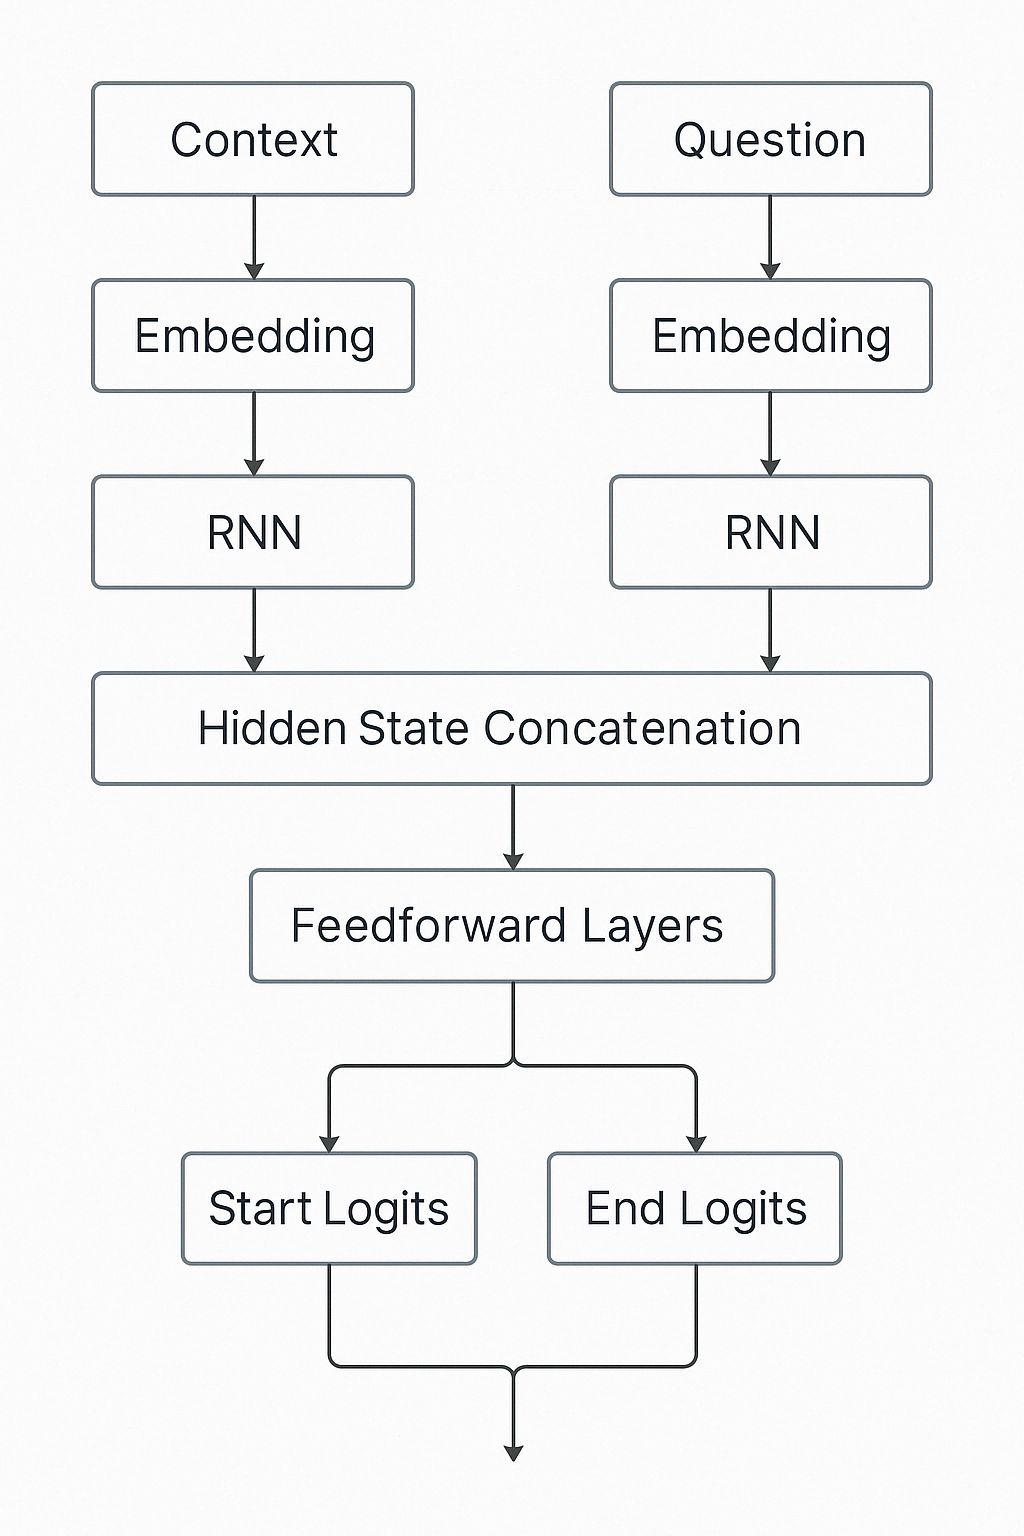
\includegraphics[width=0.4\textwidth]{images/model1.png}
\end{center}

\subsubsection{Input \& Output}
\begin{itemize}
    \item \textbf{Inputs}:
    \begin{itemize}
        \item \texttt{context (LongTensor)}: Tokenized context sequence.
        \item \texttt{question (LongTensor)}: Tokenized question sequence.
    \end{itemize}
    \item \textbf{Outputs}:
    \begin{itemize}
        \item \texttt{start\_logits}, \texttt{end\_logits}: Logits over the context, computed from the combined hidden states.
    \end{itemize}
\end{itemize}

\subsubsection{Model Highlights}
\begin{itemize}
    \item Summarizes the entire context and question into single fixed-size vectors before answer prediction.
    \item Lightweight and efficient; serves as a baseline for comparing attention-based mechanisms.
    \item Supports configurable RNN types and optional pretrained embeddings.
\end{itemize}

\subsection{Cross-Attention Transformer Model}

This model adopts an approach inspired by encoder-decoder architectures, specifically focusing on enriching the context representation by attending to the question.

\subsubsection{Architecture Overview}
\begin{itemize}
    \item \textbf{Embedding Layer}: Context and question tokens are independently embedded with token and positional embeddings. Dropout is applied.
    \item \textbf{Question Encoder}: Embedded question is passed through a Transformer Encoder block.
    \item \textbf{Cross-Attention Layers}: Context representations act as queries, and the encoded question representations act as keys and values.
    \item \textbf{Output Heads}: The final context representations are passed through linear layers to produce start and end logits.
    \item \textbf{Masking}: Padding tokens are masked in both context and question during attention computations.
\end{itemize}

\subsubsection{Input \& Output}
\begin{itemize}
    \item \textbf{Inputs}:
    \begin{itemize}
        \item \texttt{context (LongTensor)}
        \item \texttt{question (LongTensor)}
        \item \texttt{attention\_mask\_context (Tensor)} (optional)
        \item \texttt{attention\_mask\_question (Tensor)} (optional)
    \end{itemize}
    \item \textbf{Outputs}:
    \begin{itemize}
        \item \texttt{start\_logits}, \texttt{end\_logits}
    \end{itemize}
\end{itemize}

\subsubsection{Model Highlights}
\begin{itemize}
    \item Uses cross-attention to model fine-grained interaction between context and question.
    \item Properly masks padding tokens.
    \item Modular configuration of attention layers and Transformer blocks.
    \item Residual connections and layer normalization ensure stable training.
\end{itemize}

\subsection{DrQA-Inspired BiLSTM Model} \cite{drqa}

This model is a simplified version of the DrQA Document Reader. It uses separate BiLSTM encoders for the question and context, followed by a dot-product attention mechanism and a pointer network.

\subsubsection{Architecture Overview}
\begin{itemize}
    \item \textbf{Embedding Layer}: Maps tokens to dense vectors; handles padding.
    \item \textbf{BiLSTM Encoders}: Encode context and question independently with 3-layer BiLSTM networks.
    \item \textbf{Dot-Product Attention}: Computes a similarity matrix between context and question encodings.
    \item \textbf{Fusion Layer}: Concatenates attention-weighted question vectors with context representations.
    \item \textbf{Pointer Network}: Uses MLPs to predict start and end positions.
\end{itemize}

\subsubsection{Input \& Output}
\begin{itemize}
    \item \textbf{Inputs}:
    \begin{itemize}
        \item \texttt{context (LongTensor)}
        \item \texttt{question (LongTensor)}
        \item \texttt{attention\_mask\_question (Tensor)} (optional)
    \end{itemize}
    \item \textbf{Outputs}:
    \begin{itemize}
        \item \texttt{start\_logits}, \texttt{end\_logits}
    \end{itemize}
\end{itemize}

\subsubsection{Model Highlights}
\begin{itemize}
    \item Uses dot-product attention for fine-grained alignment.
    \item Masks question padding tokens.
    \item Lightweight and avoids early summarization of input.
\end{itemize}

\subsection{Bi-Directional Attention Flow (BiDAF) Model}  \cite{bidaf}

The BiDAF model explicitly models the interaction between context and question using bi-directional attention mechanisms.

\subsubsection{Architecture Overview}
\begin{itemize}
    \item \textbf{Embedding Layer}: Converts word indices to vectors using an embedding layer (optionally pretrained).
    \item \textbf{Contextual Encoder}: BiLSTM encodes context and question sequences independently.
    \item \textbf{Attention Flow Layer}:
    \begin{itemize}
        \item \textbf{Context-to-Query (C2Q)} Attention
        \item \textbf{Query-to-Context (Q2C)} Attention
        \item Combines original and attended vectors to form augmented representation $G$.
    \end{itemize}
    \item \textbf{Modeling Layer}: 2-layer BiLSTM processes $G$ to produce refined representation $M$.
    \item \textbf{Output Layer}: Combines $G$, $M$, and $M_2$ to compute logits via linear layers.
\end{itemize}

\subsubsection{Input \& Output}
\begin{itemize}
    \item \textbf{Inputs}:
    \begin{itemize}
        \item \texttt{context (Tensor)}: $(\text{batch}, c\_len)$
        \item \texttt{question (Tensor)}: $(\text{batch}, q\_len)$
    \end{itemize}
    \item \textbf{Outputs}:
    \begin{itemize}
        \item \texttt{start\_logits}, \texttt{end\_logits}
    \end{itemize}
\end{itemize}

\subsubsection{Model Highlights}
\begin{itemize}
    \item Uses both C2Q and Q2C attention to focus on relevant parts of input.
    \item Modular and extensible architecture.
    \item Handles variable-length inputs with proper masking.
    \item Residual connections and dropout improve training stability.
\end{itemize}

\subsection{Transformer-Encoder QA Model with GloVe Embeddings}

We implemented a transformer-based question answering model, \texttt{TransformerQAModel3}, tailored for extractive QA tasks. This architecture encodes a concatenated sequence of the question and context and predicts the start and end positions of the answer span within the context.

\subsubsection{Architecture Overview}
\begin{itemize}
    \item \textbf{Embedding Layer}: The model begins with a token embedding layer initialized using pretrained GloVe embeddings. These embeddings provide semantically rich representations and can optionally be frozen during training.
    \item \textbf{Positional Encoding}: Learnable positional embeddings are added to the token embeddings to provide the model with positional information, which transformers lack inherently.
    \item \textbf{Transformer Encoder}: The main component of the model is a stack of Transformer encoder layers. Each layer includes multi-head self-attention and a feed-forward network, along with layer normalization and residual connections, allowing the model to capture global contextual relationships across the entire sequence.
    \item \textbf{Dropout Layer}: Dropout is applied to both the embeddings and transformer outputs to reduce overfitting during training.
    \item \textbf{Prediction Heads}: Two independent linear layers compute logits for the start and end positions of the answer. These operate over the final encoded representation of the context tokens only.
\end{itemize}

\subsubsection{Input \& Output}
\begin{itemize}
    \item \textbf{Inputs}:
    \begin{itemize}
        \item \texttt{context\_question} $(\in \mathbb{Z}^{B \times L})$: Concatenated tokenized question and context sequence. $B$ is the batch size, $L = m + n - 1$ is the total sequence length (where $m$ and $n$ are the max lengths of the question and context).
        \item \texttt{attention\_mask\_context\_question} $(\in \{0,1\}^{B \times L})$: A binary mask indicating valid tokens (1) and padding tokens (0), used during attention calculations.
    \end{itemize}
    \item \textbf{Outputs}:
    \begin{itemize}
        \item \texttt{start\_logits} $(\in \mathbb{R}^{B \times n})$: Unnormalized scores for each context token, indicating likelihood of being the start of the answer span.
        \item \texttt{end\_logits} $(\in \mathbb{R}^{B \times n})$: Similar logits indicating the end of the answer span.
    \end{itemize}
\end{itemize}

\subsubsection{Model Highlights}
\begin{itemize}
    \item Utilizes pretrained GloVe embeddings with optional freezing to preserve linguistic priors.
    \item Employs learnable positional embeddings to encode sequence order.
    \item Uses a stacked Transformer encoder to capture long-range dependencies in the input.
    \item Predicts start and end logits over the context tokens only, ensuring extraction from the passage.
    \item Supports attention masking for variable-length sequences and padding handling.
\end{itemize}


\section{Training Procedure}
\subsection{Training Configuration}

All four models were trained using the same configuration for consistency and fair comparison. The training setup is as follows:

\begin{itemize}
    \item \textbf{Optimizer:} AdamW
    \item \textbf{Learning Rate:} 0.001
    \item \textbf{Batch Size:} 32 or 64, depending on memory availability
    \item \textbf{Number of Epochs:} 20
    \item \textbf{Dropout Rate:} 0.1
    \item \textbf{Early Stopping:} Training was stopped early if no improvement in validation loss was observed for 5 consecutive epochs.
    \item \textbf{Learning Rate Scheduler:} The learning rate was reduced by a factor of 0.1 if validation performance did not improve for 2 consecutive epochs.
\end{itemize}

\subsection{Loss Function}

We used the Cross-Entropy Loss to train all models, implemented as \texttt{nn.CrossEntropyLoss} in PyTorch. Since the task is formulated as predicting the start and end token positions of the answer span within the context, we compute the cross-entropy loss separately for both the start and end positions. The final loss is the sum of the two individual losses:

\begin{equation}
\mathcal{L}_{\text{total}} = \mathcal{L}_{\text{start}} + \mathcal{L}_{\text{end}}
\end{equation}

This approach treats the prediction of the start and end indices as two separate multi-class classification tasks over the sequence length of the context.

\subsection{Evaluation Metrics}

To evaluate our models, we used a variety of metrics that assess performance at both the token and span levels. Each of the following metrics is computed independently for the \textbf{start} and \textbf{end} positions of the predicted answer span, allowing us to monitor their convergence during training:

\begin{itemize}
    \item \textbf{Start Accuracy \& End Accuracy:} 
    These metrics measure the proportion of correct predictions for the start and end positions, respectively. Monitoring both allows us to observe how well the model learns to identify each boundary of the answer span.

    \item \textbf{Start Precision \& End Precision:}
    Precision is computed separately for start and end positions as the fraction of predicted positions that match the true start or end token.

    \item \textbf{Start Recall \& End Recall:}
    Recall reflects how many of the true start or end tokens were correctly predicted. This metric is also tracked individually for both positions.

    \item \textbf{Start F1 Score \& End F1 Score:}
    The harmonic mean of precision and recall, providing a balanced measure of model performance for both the start and end token predictions.

    \item \textbf{Joint Exact Match (EM):}
    This metric indicates the percentage of predictions where \textit{both} the start and end positions exactly match the ground truth span. It is a strict metric for measuring exact span extraction accuracy.

    \item \textbf{Span Overlap F1:}
    A more lenient metric that measures the F1 score based on the overlap between the predicted and ground truth spans, treating both as sets of tokens. This metric captures partial correctness in span prediction.
\end{itemize}

All metrics were tracked across training epochs to assess convergence and guide model selection.


\section{Evaluation}

We evaluate our models using standard metrics for extractive question answering: start and end accuracy, precision, recall, F1-score, joint exact match (EM), and span overlap F1. The results for both training and testing datasets are presented in the following tables.

\subsection{Results}

As shown, the BiDAF and DrQA models significantly outperform the others in both training and validation metrics. BiDAF achieves high training performance, maintaining decent generalization on the validation set with a joint exact match (EM) of 0.4515 and span F1 of 0.5215. DrQA performs slightly better on training but generalizes slightly worse than BiDAF.
\\
\par
In contrast, the Glove Transformer and RNN-based models (especially the Context Separated variant) perform poorly, indicating issues in either architectural choices or their ability to capture relationships in the context-question span prediction task. The QA Separated Transformer shows some promise but still lags behind the more traditional attention-based architectures like BiDAF.
\\
\par
This reinforces the effectiveness of combining attention with recurrent mechanisms (as in BiDAF), particularly in tasks requiring precise span detection like extractive QA.
\\
\par

\begin{table}[H] % Use [H] from the float package for exact placement
\centering
\caption{Training evaluation metrics for all models}
\label{tab:train-results}
\resizebox{\textwidth}{!}{% Add % to avoid spurious space
\begin{tabular}{|l|c|c|c|c|c|c|c|c|c|c|} % Added | for vertical borders
\hline % Replaced \toprule with \hline
\textbf{Model} & \textbf{\makecell{Start\\Acc}} & \textbf{\makecell{End\\Acc}} & \textbf{\makecell{Start\\F1}} & \textbf{\makecell{End\\F1}} & \textbf{\makecell{Start\\Prec}} & \textbf{\makecell{End\\Prec}} & \textbf{\makecell{Start\\Rec}} & \textbf{\makecell{End\\Rec}} & \textbf{\makecell{Joint\\EM}} & \textbf{\makecell{Span\\F1}} \\
\hline % Replaced \midrule with \hline
BiDAF & 0.83 & 0.83 & 0.83 & 0.83 & 0.84 & 0.84 & 0.83 & 0.83 & 0.80 & 0.83 \\
\hline % Added \hline for separation
DrQA & 0.84 & 0.83 & 0.84 & 0.83 & 0.84 & 0.84 & 0.84 & 0.83 & 0.80 & 0.82 \\
\hline % Added \hline for separation
GloVe Transformer & 0.26 & 0.26 & 0.26 & 0.27 & 0.26 & 0.27 & 0.26 & 0.26 & 0.22 & 0.23 \\
\hline % Added \hline for separation
RNN Context Sep. & 0.06 & 0.05 & 0.02 & 0.02 & 0.02 & 0.02 & 0.06 & 0.05 & 0.03 & 0.06 \\
\hline % Added \hline for separation
QA Transformer Sep. & 0.18 & 0.20 & 0.17 & 0.19 & 0.19 & 0.22 & 0.18 & 0.20 & 0.09 & 0.12 \\
\hline % Replaced \bottomrule with \hline
\end{tabular}% Add % to avoid spurious space
}
\end{table}
% No vertical space command here ensures minimal gap
\begin{table}[H] % Use [H] from the float package for exact placement
\centering
\caption{Testing evaluation metrics for all models}
\label{tab:test-results}
\resizebox{\textwidth}{!}{% Add % to avoid spurious space
\begin{tabular}{|l|c|c|c|c|c|c|c|c|c|c|} % Added | for vertical borders
\hline % Replaced \toprule with \hline
\textbf{Model} & \textbf{\makecell{Start\\Acc}} & \textbf{\makecell{End\\Acc}} & \textbf{\makecell{Start\\F1}} & \textbf{\makecell{End\\F1}} & \textbf{\makecell{Start\\Prec}} & \textbf{\makecell{End\\Prec}} & \textbf{\makecell{Start\\Rec}} & \textbf{\makecell{End\\Rec}} & \textbf{\makecell{Joint\\EM}} & \textbf{\makecell{Span\\F1}} \\
\hline % Replaced \midrule with \hline
BiDAF & 0.52 & 0.51 & 0.52 & 0.51 & 0.54 & 0.54 & 0.52 & 0.51 & 0.45 & 0.52 \\
\hline % Added \hline for separation
DrQA & 0.28 & 0.28 & 0.28 & 0.27 & 0.30 & 0.29 & 0.28 & 0.28 & 0.24 & 0.27 \\
\hline % Added \hline for separation
GloVe Transformer & 0.13 & 0.13 & 0.13 & 0.13 & 0.14 & 0.15 & 0.13 & 0.13 & 0.11 & 0.12 \\
\hline % Added \hline for separation
RNN Context Sep. & 0.03 & 0.03 & 0.01 & 0.01 & 0.01 & 0.01 & 0.03 & 0.03 & 0.01 & 0.04 \\
\hline % Added \hline for separation
QA Transformer Sep. & 0.11 & 0.11 & 0.10 & 0.10 & 0.12 & 0.12 & 0.11 & 0.11 & 0.05 & 0.08 \\
\hline % Replaced \bottomrule with \hline
\end{tabular}% Add % to avoid spurious space
}
\end{table}

\subsection{Qualitative Examples of Correct Predictions}

Below are some selected examples from the validation set.

\subsubsection*{RNN Seperated}

\begin{itemize}
  \item \textbf{Question:} \textit{How many Khitan tumens were there?}
  \item \textbf{Context (excerpt):} \textit{... there were 4 Han tumens and 3 Khitan tumens, with each tumen consisting of 10,000 troops ...}
  \item \textbf{Predicted Answer:} \texttt{3}
  \item \textbf{True Answer:} \texttt{3}
\end{itemize}
\begin{itemize}
  \item \textbf{Question:} \textit{What is the atomic number of the element oxygen?}
  \item \textbf{Context (excerpt):} \textit{... oxygen is a chemical element with symbol O and atomic number 8 ...}
  \item \textbf{Predicted Answer:} \texttt{and atomic}
  \item \textbf{True Answer:} \texttt{8}
\end{itemize}

\subsubsection{QA Transformer Seperated}

\begin{itemize}
  \item \textbf{Question:} \textit{How many Khitan tumens were there?}
  \item \textbf{Context (excerpt):} \textit{... there were 4 Han tumens and 3 Khitan tumens, with each tumen consisting of 10,000 troops ...}
  \item \textbf{Predicted Answer:} \texttt{3}
  \item \textbf{True Answer:} \texttt{3}
\end{itemize}

\begin{itemize}
  \item \textbf{Question:} \textit{What is the atomic number of the element oxygen?}
  \item \textbf{Context (excerpt):} \textit{... oxygen is a chemical element with symbol O and atomic number 8 ...}
  \item \textbf{Predicted Answer:} \texttt{20.8\%}
  \item \textbf{True Answer:} \texttt{8}
\end{itemize}

\subsubsection{GloVe Transformer}

\begin{itemize}
    \item \textbf{Question:} \textit{How many Khitan tumens were there?}
    \item \textbf{Context (excerpt):} \textit{... there were 4 Han tumens and 3 Khitan tumens, with each tumen consisting of 10,000 troops ...}
    \item \textbf{Predicted Answer:} \texttt{3}
    \item \textbf{True Answer:} \texttt{3}
\end{itemize}

\begin{itemize}
    \item \textbf{Question:} \textit{What is the atomic number of the element oxygen?}
    \item \textbf{Context (excerpt):} \textit{... oxygen is a chemical element with symbol O and atomic number 8 ...}
    \item \textbf{Predicted Answer:} \texttt{oxygen}
    \item \textbf{True Answer:} \texttt{8}
\end{itemize}

  
\subsubsection{BiDAF}
\begin{itemize}
    \item \textbf{Question:} \textit{How many Khitan tumens were there?}
    \item \textbf{Context (excerpt):} \textit{... there were 4 Han tumens and 3 Khitan tumens, with each tumen consisting of 10,000 troops ...}
    \item \textbf{Predicted Answer:} \texttt{3}
    \item \textbf{True Answer:} \texttt{3}
\end{itemize}

\begin{itemize}
    \item \textbf{Question:} \textit{What is the atomic number of the element oxygen?}
    \item \textbf{Context (excerpt):} \textit{... oxygen is a chemical element with symbol O and atomic number 8 ...}
    \item \textbf{Predicted Answer:} \texttt{8}
    \item \textbf{True Answer:} \texttt{8}
\end{itemize}
  
\subsubsection{DrQA}

\begin{itemize}
    \item \textbf{Question:} \textit{How many Khitan tumens were there?}
    \item \textbf{Context (excerpt):} \textit{... there were 4 Han tumens and 3 Khitan tumens, with each tumen consisting of 10,000 troops ...}
    \item \textbf{Predicted Answer:} \texttt{two}
    \item \textbf{True Answer:} \texttt{3}
\end{itemize}

\begin{itemize}
    \item \textbf{Question:} \textit{What is the atomic number of the element oxygen?}
    \item \textbf{Context (excerpt):} \textit{... oxygen is a chemical element with symbol O and atomic number 8 ...}
    \item \textbf{Predicted Answer:} \texttt{8}
    \item \textbf{True Answer:} \texttt{8}
\end{itemize}

All models predicted the correct answer for the \textit{Khitan tumens} question except \textbf{DrQA}, which predicted \texttt{two} instead of \texttt{3}.  
All models failed on the \textit{atomic number of oxygen} question except \textbf{BiDAF} and \textbf{DrQA}, which predicted the correct answer \texttt{8}.

\subsection{Learning Curves}

\subsubsection*{RNN Separated}
Figure~\ref{fig:rnn_loss} shows the training and validation loss over 9 epochs. The training loss keeps going down, which means the model is learning from the training data.

However, the validation loss starts increasing after around the 4th epoch. This means the model is starting to overfit — it performs well on training data but worse on unseen data.

This training was originally planned for 20 epochs, but it stopped early because of early stopping. Dropout and learning rate scheduling were also used to reduce overfitting, but the model still started to overfit after a few epochs. This suggests the model may need further tuning or regularization.
\begin{figure}[H]
\centering
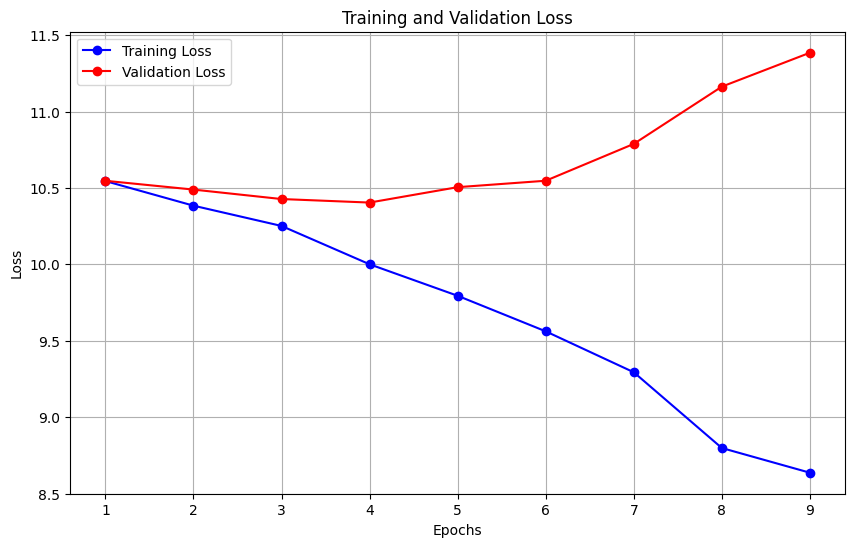
\includegraphics[width=0.8\textwidth]{images/rnn_loss.png}
\caption{Learning curves for the RNN Separated model showing training and validation loss.}
\label{fig:rnn_loss}
\end{figure}

\subsubsection*{QA Transformer Separated}
Figure~\ref{fig:qa2_loss} shows the training and validation loss over 6 epochs. The training loss decreases steadily, which means the model is learning well on the training data.

However, the validation loss increases after the second epoch and becomes much higher than the training loss. This suggests the model starts to overfit very early — it memorizes the training data but does not perform well on new data.

Even though early stopping and other techniques were likely used, the gap between training and validation loss shows the model struggles to generalize. This might be due to a small dataset, high model complexity, or not enough regularization.
\begin{figure}[H]
\centering
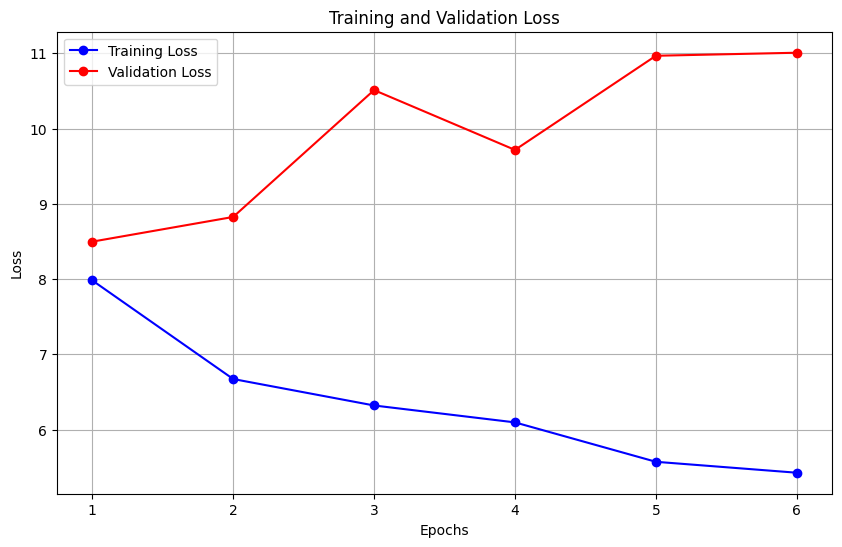
\includegraphics[width=0.8\textwidth]{images/qa2_loss.png}
\caption{Learning curves for the QA Transformer Separated model showing training and validation loss.}
\label{fig:qa_transformer_loss}
\end{figure}

\subsubsection*{GloVe Transformer}
Figure~\ref{fig:qa3_loss} illustrates the training and validation loss over 10 epochs. The training loss shows a consistent downward trend, indicating that the model is learning effectively on the training data.

In contrast, the validation loss fluctuates throughout training and does not show clear improvement. After a slight decrease in the early epochs, it remains relatively high and even increases in later epochs, suggesting that the model is overfitting — it continues to fit the training data better while failing to improve on unseen data.

This pattern indicates poor generalization and may be due to insufficient regularization, overly complex architecture, or limitations in the dataset size or diversity. Despite the extended training duration, the persistent gap between training and validation losses emphasizes the need for strategies like stronger regularization, simpler models, or data augmentation.
\begin{figure}[H]
\centering
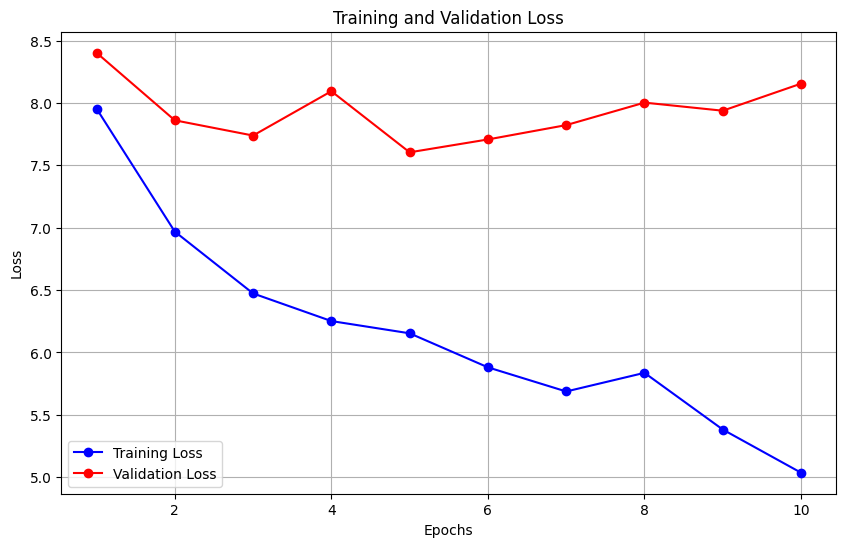
\includegraphics[width=0.8\textwidth]{images/qa3_loss.png}
\caption{Learning curves for the GloVe Transformer model showing training and validation loss.}
\label{fig:glove_transformer_loss}
\end{figure}

\subsubsection*{BiDAF}
Figure~\ref{fig:bidaf_loss} presents the training and validation loss over 8 epochs. The training loss shows a sharp and consistent decline, suggesting that the model is effectively minimizing error on the training set.

In contrast, the validation loss initially decreases slightly but then begins to rise steadily from the fourth epoch onward. By the final epochs, the gap between training and validation loss becomes significant, indicating that the model is overfitting. It continues to improve on the training data while its performance on unseen data worsens.

This pattern implies a lack of generalization and highlights the importance of applying stronger regularization techniques or introducing early stopping. It may also suggest that the model is too complex for the size or diversity of the dataset used.
\begin{figure}[H]
\centering
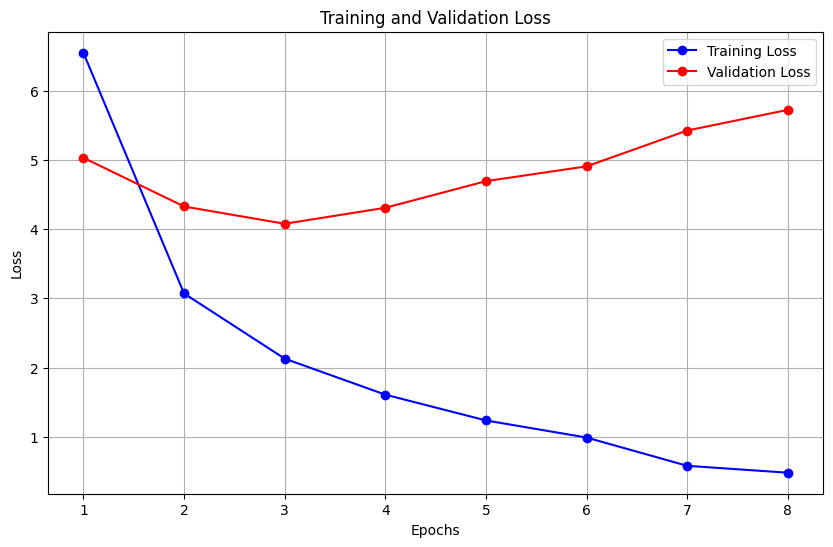
\includegraphics[width=0.8\textwidth]{images/bidaf_loss.png}
\caption{Learning curves for the BiDAF model showing training and validation loss.}
\label{fig:bidaf_loss}
\end{figure}

\subsubsection*{DrQA}
Figure~\ref{fig:drqa_loss} shows the training and validation loss across 7 epochs. The training loss decreases consistently, indicating that the model is learning to minimize error on the training set.

However, the validation loss starts to diverge significantly from the training loss after the third epoch. It rises steadily and sharply in the later epochs, suggesting strong overfitting — the model is adapting too well to the training data and failing to generalize to unseen data.

This pattern points to issues such as an overly complex model, inadequate regularization, or a training set that does not represent the validation set well. The rapid rise in validation loss highlights the need for earlier stopping, dropout, or possibly simplifying the model architecture to prevent overfitting.
\begin{figure}[H]
\centering
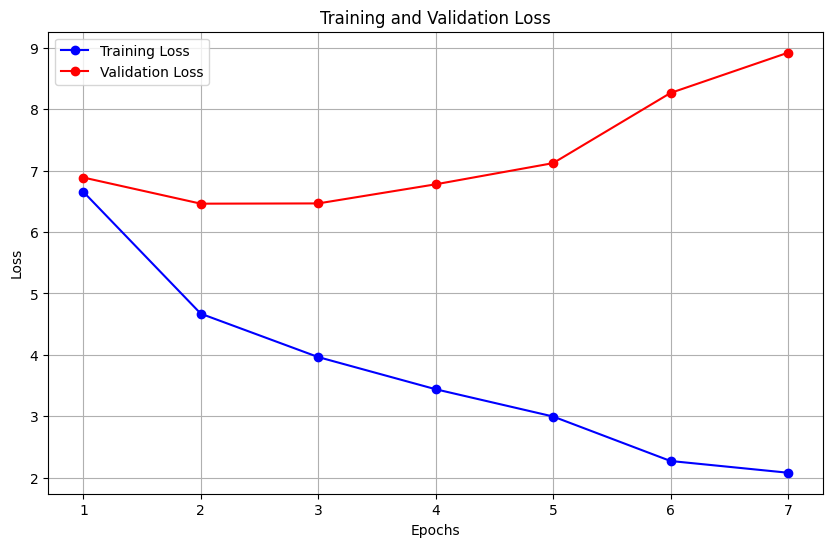
\includegraphics[width=0.8\textwidth]{images/drqa_loss.png}
\caption{Learning curves for the DrQA model showing training and validation loss.}
\label{fig:drqa_loss}
\end{figure}
\section{Discussion}
The results highlight a significant disparity in performance across the different model architectures we experimented with. The BiDAF model stands out as the most effective, achieving the highest scores on both the joint exact match and span F1 metrics on the validation set. This suggests that the bi-directional attention mechanism is particularly well-suited for capturing the nuanced interactions between the question and the context required for accurate span prediction. The DrQA-inspired model also shows reasonable performance, indicating the value of combining BiLSTMs with an attention mechanism.

In contrast, the models that process the question and context more independently or rely solely on a Transformer encoder with GloVe embeddings struggled to achieve comparable results. The poor performance of the Dual-RNN model underscores the limitation of summarizing the entire context and question into fixed-size vectors without a more fine-grained interaction mechanism. Similarly, the weaker results from the GloVe Transformer and the QA Separated Transformer suggest that without more sophisticated architectural adaptations or pre-training on larger datasets, these models may not effectively learn the complex relationships needed for precise answer extraction in our limited data setting.

It is also worth noting the differences between training and validation performance. While some models achieved high scores on the training data, their performance dropped on the validation set, indicating potential overfitting. The BiDAF model showed a relatively smaller gap between training and validation scores, suggesting better generalization capabilities.

\section{Limitations}

Our project faced several limitations that likely impacted the performance of our models:

\begin{itemize}
    \item \textbf{Limited Dataset Size:} Using only 20,000 answerable examples from the SQuAD 2.0 dataset is a significant reduction from the full dataset. This smaller size likely limited the ability of more complex models, especially the transformer-based ones, to learn robust representations and generalize well.
    
    \item \textbf{Restricted Model Complexity:} The constraint of using only three layers (excluding input and output) limited the depth and capacity of our models. Deeper networks, particularly in transformer architectures, often benefit from their ability to learn hierarchical features.
    
    \item \textbf{Computational Resources:} Limited access to high-end GPUs restricted the batch sizes, training times, and the ability to experiment with larger or more computationally intensive models. This also constrained our ability to perform extensive hyperparameter tuning.
    
    \item \textbf{Model Architecture Constraints:} The instruction to use either RNN-based or attention-based models, but not a combination (initially), prevented us from fully exploring architectures that the literature suggests are highly effective, such as those combining RNNs with attention mechanisms. While we did implement BiDAF which does this, our exploration of other hybrid models was limited.
    
    \item \textbf{Data Filtering:} Filtering the dataset based on context length, while helpful for managing computational resources, might have introduced biases or excluded valuable examples that could have improved model generalization.
    
    \item \textbf{Tokenization and Vocabulary Size:} Our choice of a 10,000 subword vocabulary using BPE might not have been optimal. Exploring different tokenization strategies or vocabulary sizes could potentially impact performance.
    
    \item \textbf{Lack of Pre-training:} Except for the GloVe embeddings used in one of the transformer models, our models were trained from scratch on the limited SQuAD subset. Leveraging large pre-trained language models like BERT, even with fine-tuning on our smaller dataset, could have significantly boosted performance.
    
    \item \textbf{Evaluation Metrics Focus:} While we used standard evaluation metrics, focusing solely on exact match and F1 score might not fully capture the nuances of the generated answers. Other metrics, such as those evaluating semantic similarity, could provide a more comprehensive understanding of the model's capabilities.
\end{itemize}

These limitations highlight areas for potential improvement in future work, such as utilizing the full SQuAD dataset, experimenting with deeper and more complex architectures (if computational resources allow), leveraging pre-trained models, and exploring different data preprocessing and tokenization techniques.



	
	\bibliographystyle{apalike}
	\bibliography{mybib}
	
\end{document}
